%!TEX root = ../thesis.tex
%*******************************************************************************
%****************************** Second Chapter *********************************
%*******************************************************************************

\chapter{Methodology}

\ifpdf
    \graphicspath{{Chapter2/Figs/Raster/}{Chapter2/Figs/PDF/}{Chapter2/Figs/}{Chapter2/Figures/}}
\else
    \graphicspath{{Chapter2/Figs/Vector/}{Chapter2/Figs/}{Chapter2/Figures/}}
\fi

This section describes how the sources of uncertainty in PILCO's decision making process are disentangled and quantified. First, section \ref{S:PILCO} provides a brief introduction to the PILCO algorithm. In Section \ref{S:approximating-pilcos-gp} a finite-weight trigonometric Bayesian regression model is introduced to approximate PILCO's probabilistic Gaussian Process (GP) dynamics model. Section \ref{S:sparse-approximation} relates the trigonometric model to a full GP by showing that it can be interpreted as sparse spectrum GP that can approximate any full GP. The sources of uncertainty in transition function and their effect on the cost are discussed in section \ref{S:disentangling-uncertainty} and a variance decomposition to separate and quantify the uncertainty into its aleatoric and epistemic constituents is presented. Finally, section \ref{S:monte-carlo-estimate} presents a "gold-standard" Monte-Carlo scheme to estimate the aleatoric and epistemic uncertainties. 

\section{PILCO}
\label{S:PILCO}
PILCO \citep{deisenroth2011pilco} is a model-based indirect policy search method for continuous state $\mathbf{x} \in \mathbb{R}^{D}$ and action $\mathbf{u} \in \mathbb{R}^{F}$ dynamical systems described by
\begin{equation}
    \mathbf{x}_{t+1}=f\left(\mathbf{x}_{t}, \mathbf{u}_{t}\right)+\mathbf{\eta}, \quad \mathbf{\eta} \sim \mathcal{N}\left(\mathbf{0}, \boldgreek{\Sigma}_{\eta}\right)
\end{equation}
where the transition dynamics $f$ of the system are unknown. The objective is to find a deterministic \textit{controller/policy} $\pi : \mathbf{x} \mapsto \pi(\mathbf{x}, \boldgreek{\theta})=\mathbf{u}$ such that the expected return   \citep{deisenroth2013gaussian}
\begin{equation}
    J^{\pi}(\theta)=\sum_{t=0}^{T} \mathbb{E}_{\mathbf{x}_{t}}\left[\mathbb{C}\left(\mathbf{x}_{t}\right)\right], \quad \mathbf{x}_{0} \sim \mathcal{N}\left(\boldgreek{\mu}_{0}, \boldgreek{\Sigma}_{0}\right)
    \label{Eq:PILCO-expected-return}
\end{equation}
is minimised after following $\pi$ for $T$ steps. The policy is parametrised by $\mathbf{\theta}$, which take the form of nonlinear RBF networks, where $\mathbf{\theta}$ are the weights and features, or linear-affine transformations, where $\mathbf{\theta}$ are the weights matrix and bias terms. The \textit{cost} $\mathbb{C}(\mathbf{x}_{t})$, or negative reward, of being in state $\mathbf{x}$ at time $t$ is the generalised binary saturating cost \citep{deisenroth2013gaussian}
\begin{equation}
    \mathbb{C}(\mathbf{x}_{t})=1-\exp \left(-\frac{1}{2 \sigma_{c}^{2}} ||\mathbf{x}_{t}- \mathbf{x}_{\text { target }}||^{2}\right) \in[0,1]
    \label{Eq:PILCO-cost-function}
\end{equation}
which exclusively penalises the Euclidean distance $||\mathbf{x}_{t}- \mathbf{x}_{\text { target }}||^{2}$ from the current state $\mathbf{x}_{t}$ to the target state $\mathbf{x}_{\text { target }}$. $\mathbb{C}(\mathbf{x}_{t})$ is locally quadratic and saturates at 1 for large differences between the current state and target state. The saturation distance is controlled by the width parameter $\sigma_{c}$.

\subsection{GP Model Learning}
\label{PILCO:GP-model-learning}
The system dynamics are modelled as a probabilistic Gaussian Process (GP). Tuples of the state and control vectors $\left(\mathbf{x}_{t}, \mathbf{u}_{t}\right)\in \mathbb{R}^{D+F}$ serve as training inputs and differences $\Delta_{t}=\mathbf{x}_{t+1}-\mathbf{x}_{t}+\varepsilon \in \mathbb{R}^{D},\quad \varepsilon \sim \mathcal{N}\left(0, \boldgreek{\Sigma}_{\varepsilon}\right)$ as training targets. Conditionally independent GP's are trained for each target dimension \citep{deisenroth2010efficient}. The dynamics model provides a \textit{one-step} prediction \citep{deisenroth2011pilco}
\begin{equation}
    p\left(\mathbf{x}_{t+1} | \mathbf{x}_{t}, \mathbf{u}_{t}\right)=\mathcal{N}\left(\mathbf{x}_{t} | \mu_{t}, \boldgreek{\Sigma}_{t}\right)
    \label{Eq:PILCO-one-step-1}
\end{equation}
\begin{equation}
    \mu_{t+1}=\mathbf{x}_{t}+\mathbb{E}_{f}\left[\Delta_{t}\right]
    \label{Eq:PILCO-one-step-2}
\end{equation}
\begin{equation}
    \boldgreek{\Sigma}_{t+1}=\operatorname{var}_{f}\left[\Delta_{t}\right]
    \label{Eq:PILCO-one-step-3}
\end{equation}
where the mean $\mu$ of the state $\mathbf{x}_{t+1}$ is obtained through addition of the current state $\mathbf{x}_{t}$ with the one-step difference prediction $\mathbb{E}_{f}\left[\Delta_{t}\right]$. A GP is defined completely by a mean function $m(\cdot)$ and a positive semidefinite covariance function $K(\cdot,\cdot)$. PILCO follows the common practice of setting the mean prior function to zero and uses the \textit{stationary} anisotropic squared exponential covariance function
\begin{equation}
    k\left(\tilde{\mathbf{x}}_{i}, \tilde{\mathbf{x}}_{j}\right)=\sigma_{0}^{2} \exp \left(-\frac{1}{2}\left(\tilde{\mathbf{x}}_{i}-\tilde{\mathbf{x}}_{j}\right)^{\top} \boldgreek{\Lambda}^{-1}\left(\tilde{\mathbf{x}}_{i}-\tilde{\mathbf{x}}_{j}\right)\right)
    \label{Eq:PILCO-sq-exponential-covariance}
\end{equation}
where $\tilde{\mathbf{x}} = \left[\mathbf{x}\quad\mathbf{u}\right]^{T}$ is the state-action vector, $\boldgreek{\Lambda} =\operatorname{diag}\left(\left[\ell_{1}^{2}, \ldots, \ell_{D+F}^{2}\right]\right)$ depends on the characteristic lengthscales and $\sigma_{0}$ is the variance of the latent function \citep{deisenroth2013gaussian}. The lengthscales determine the speed that the covariance decays with the distance between inputs \citep{quia2010sparse}.

\subsection{Policy Evaluation}
\label{PILCO:policy-evaluation}
PILCO evaluates a given policy by predicting the state evolution over the course of an episode. This is accomplished by propagating uncertain inputs through the dynamics model, using the one-step predictions (Eqs. \ref{Eq:PILCO-one-step-1} - \ref{Eq:PILCO-one-step-3}), to obtain $p\left(\mathbf{x}_{1} | \pi\right), \ldots, p\left(\mathbf{x}_{T} | \pi\right)$ from a given start state distribution $p\left(\mathbf{x}_{0}\right)$. Predicting $\mathbf{x}_{t+1}$ from $p(\mathbf{x}_{t})$ requires evaluation of the predictive distribution over state differences
\begin{equation}
    p\left(\Delta_{t}\right)=\iint p\left(f\left(\tilde{\mathbf{x}}_{t}\right) | \left(\tilde{\mathbf{x}}_{t}\right)\right) p\left(\tilde{\mathbf{x}}_{t}\right) \mathrm{d} f \mathrm{d} \tilde{\mathbf{x}}_{t},
    \label{Eq:PILCO-predictive-state-differences}
\end{equation}
by integrating out the random function of the GP distribution and the random variable $\tilde{\mathbf{x}}_{t}$. Here $p\left(\tilde{\mathbf{x}}_{t}\right)=p\left(\mathbf{x}_{t}, \mathbf{u}_{t}\right)$ is the joint state-action distribution. Since the predictive distribution in Eq. \ref{Eq:PILCO-predictive-state-differences} is analytically intractable for uncertain inputs, it is approximated as a Gaussian distribution using \textit{moment matching} (see Fig. \ref{Fig:moment-matching}). This approximation ensures that the state distribution is given by $p\left(\tilde{\mathbf{x}}_{t}\right)=\mathcal{N}\left(\tilde{\mathbf{x}}_{t} | \tilde{\mathbf{\mu}}_{t}, \tilde{\boldgreek{\Sigma}}_{t}\right)$ for all $t$. This, alongside the choice of cost function (Eq. \ref{Eq:PILCO-cost-function}) enables the expected return (Eq. \ref{Eq:PILCO-expected-return}) to be evaluated analytically according to
\begin{equation}
    \mathbb{E}_{\mathbf{x}_{t}}\left[c\left(\mathbf{x}_{t}\right)\right]=\int c\left(\mathbf{x}_{t}\right) \mathcal{N}\left(\mathbf{x}_{t} | \boldgreek{\mu}_{t}, \boldgreek{\Sigma}_{t}\right) \mathrm{d} \mathbf{x}_{t}
\end{equation}
for $t=1,\dots,T$.

\begin{figure}
\centering    
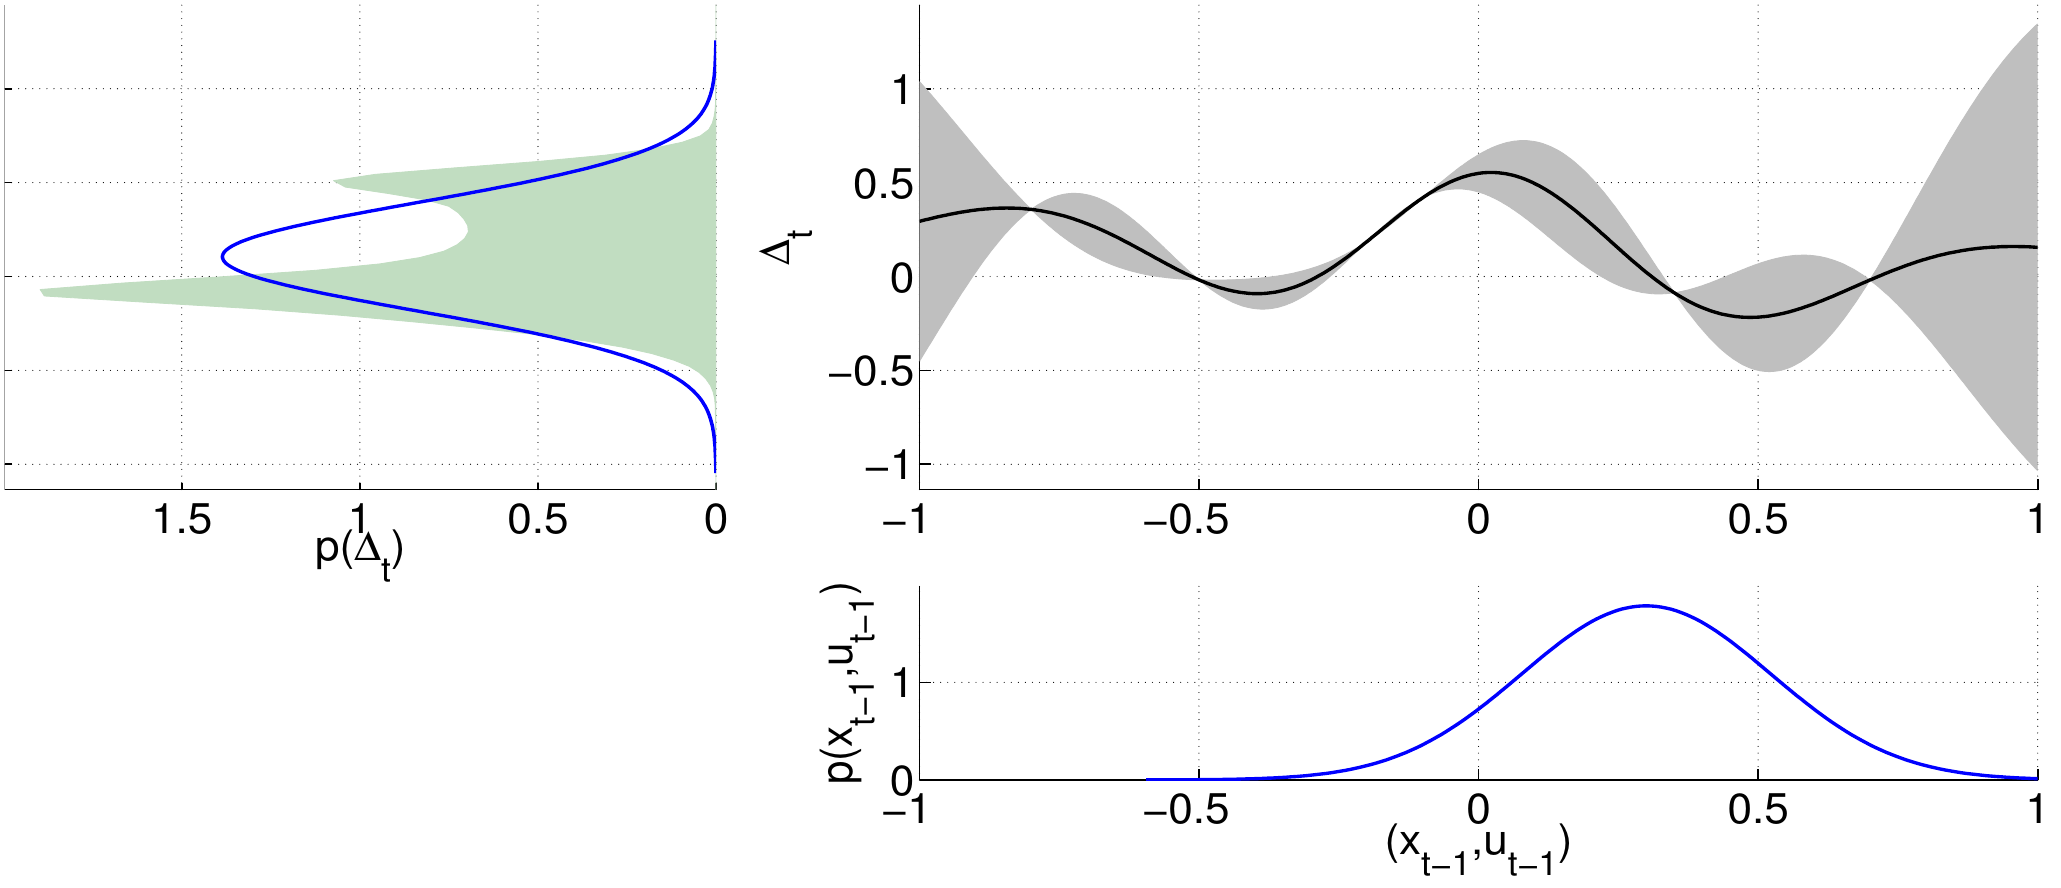
\includegraphics[width=1.0\textwidth]{PILCO-moment-matching.png}
\caption[Propagating an uncertain input through the GP dynamics model]{Propagating an uncertain input through the GP dynamics model (upper right panel). The input distribution $p(x_{t-1},u_{t-1})$, assumed to be Gaussian (lower right panel), is propagated through the dynamics model yielding the shaded distribution $p(\Delta_{t})$. The shaded distribution is then approximated by a Gaussian with the same mean and variance (upper left panel). Reproduced from \citep{deisenroth2011pilco}.}
\label{Fig:moment-matching}
\end{figure}

\subsection{Policy Improvement}
\label{PILCO:policy-improvement}
PILCO is an indirect policy search method and does not require an explicit value function model. Instead it learns a \textit{parametrised policy} that can select actions without consulting a value function. Due to the moment matching approximation, the state distribution is considered to be Gaussian $p\left(\tilde{\mathbf{x}}_{t}\right)=\mathcal{N}\left(\tilde{\mathbf{x}}_{t} | \tilde{\mathbf{\mu}}_{t}, \tilde{\boldgreek{\Sigma}}_{t}\right)$ for all $t$, where $\tilde{\mathbf{x}}_{t} = (\mathbf{x}_{t},\mathbf{u}_{t})$. The control signal  $\mathbf{u}_{t-1} = \pi\left(\mathbf{x}_{t-1}, \theta\right)$ is a function of the state, and hence the next state is also functionally dependent on the mean $\mu_{u}$ and covariance $\boldgreek{\Sigma}_{u}$ of the control signal. This relationship allows the gradients of the expected return $J^{\pi}$, with respect to the policy parameters $\boldgreek{\theta}$, to be computed analytically. The policy parameters are then learned to \textit{maximise} performance (\textit{minimise} cost) for a given task, so their updates approximate gradient \textit{descent} in $J$ \citep{sutton2018reinforcement}:
\begin{equation}
    \boldgreek{\theta}_{t+1}=\boldgreek{\theta}_{t} - \alpha\nabla J^{\pi}\left(\boldgreek{\theta_{t}}\right),
\end{equation}
where $\alpha$ is the learning rate. For a more thorough explanation of PILCO see \citep{deisenroth2011pilco}\citep{deisenroth2010efficient}\citep{deisenroth2013gaussian}. Algorithm \ref{PILCO:algorithm-1} provides an overview of PILCO.

\begin{algorithm}
\caption{Probabilistic Inference for Learning Control (PILCO)}\label{PILCO:algorithm-1}
\begin{algorithmic}[1]
\State \textbf{init:} Sample controller parameters $\boldgreek{\theta} \sim \mathcal{N}\left(\mathbf{0},\mathbf{I}\right)$
\Repeat{}
\State Learn probabilistic GP dynamics model using all environment data \Comment{Sec \ref{PILCO:GP-model-learning}}
\Repeat{}
\State Approximate inference for policy evaluation: $J^{\pi}\left(\theta\right)$ \Comment{Sec \ref{PILCO:policy-evaluation}}
\State Gradient-based policy improvement: $\mathrm{d} J^{\pi}(\boldsymbol{\theta}) / \mathrm{d} \boldsymbol{\theta}$ \Comment{Sec \ref{PILCO:policy-improvement}}
\State Update parameters $\boldgreek{\theta}$\Comment{CG or L-BFGS}
\Until convergence; \textbf{return} $\boldgreek{\theta}^{*}$
\State Set $\pi^{*} \gets \pi\left(\theta^{*}\right)$
\State  Apply $\pi^{*}$ to environment and record data
\Until task learned \Comment{modified from \citep{deisenroth2011pilco}}
\end{algorithmic}
\end{algorithm}

\section{Approximating PILCO's GP}
\label{S:approximating-pilcos-gp}
At the heart of the Monte Carlo uncertainty approximation is the need for one-step predictions using a function sampled from the posterior distribution of PILCO's dynamics model. The use of the squared exponential covariance function in PILCO's GP corresponds to a Bayesian linear regression model with an infinite number of basis functions \citep{williams2006gaussian}. This means drawing a representative function requires an infinite number of weights since each basis function is accompanied by its own weight. To overcome this issue, a finite-weight stationary trigonometric Bayesian regression model \citep{quia2010sparse} is used to approximate PILCO's GP. In addition to solving the sampling issue, this model provides other advantages. First, the periodicity of the trigonometric basis functions means that one does not need to explicitly specify the mean for each basis function. Second, a direct GP implementation has practical limitations with regards to computational and memory requirements, which scale as $\mathcal{O}(n^{2})$ and $\mathcal{O}(n^{3})$, respectively. The trigonometric model has computational requirements of $\mathcal{O}(nm^{2})$ and memory requirements of $\mathcal{O}(nm)$ where $m<<n$ \citep{quia2010sparse}, which are typical values for sparse GP approximations \citep{quinonero2005unifying}. The largest PILCO environment used for this research (cart double pendulum) generates approximately $4k$ data points. The model is first introduced here in a traditional treatment of Bayesian linear regression. Section \ref{S:one-step-predictions} relates the model to PILCO's one-step predictions. Finally, section \ref{S:sparse-approximation} shows that the model can be viewed as a sparse stationary GP that can approximate any full GP.

The model consists of a linear combination of trigonometric functions \citep{quia2010sparse}
\begin{equation}
    f(\tilde{\mathbf{x}})=\sum_{r=1}^{m} a_{r} \cos \left(2 \pi \mathbf{s}_{r}^{\top} \tilde{\mathbf{x}}\right)+b_{r} \sin \left(2 \pi \mathbf{s}_{r}^{\top} \tilde{\mathbf{x}}\right)
    \label{Eq:Model-trigonometric-model}
\end{equation}
where $\tilde{\mathbf{x}}=\left[\mathbf{x}^{\top} \ \mathbf{u}^{\top}\right]^{\top}\in\mathbb{R}^{D+F}$ is the state-action vector, $\mathbf{s}_{r}$ is a $(D+F)$-dimensional vector of spectral frequencies shared by each pair of basis functions and $a_{r}$, $b_{r}$ are amplitude parameters which are independent for each basis function (see Sec \ref{S:sparse-approximation} for selecting spectral frequencies). The amplitudes have independent Gaussian priors with linearly scaled variances 
\begin{equation}
    a_{r} \sim \mathcal{N}\left(0, \frac{\sigma_{0}^{2}}{m}\right), \quad b_{r} \sim \mathcal{N}\left(0, \frac{\sigma_{0}^{2}}{m}\right)
\end{equation}
where $m$ are the number basis functions. The frequencies function as deterministic parameters and the amplitudes are treated in a Bayesian fashion. For this, the model is packaged as the dot product between the set of amplitudes and the basis functions 
\begin{equation}
    f(\tilde{\mathbf{x}}, \mathbf{w}) = \mathbf{w}^{\top} \varphi\left(\tilde{\mathbf{x}}\right)
\end{equation}
where $\mathbf{w}=\left[a_{1}, b_{1}, \dots, a_{m}, b_{m}\right]^{\top}$ are the model weights and
\begin{equation}
    \varphi(\tilde{\mathbf{x}})=\left[\cos \left(2 \pi \mathbf{s}_{1}^{\top} \tilde{\mathbf{x}}\right)\quad \sin \left(2 \pi \mathbf{s}_{1}^{\top} \tilde{\mathbf{x}}\right) \quad\ldots\quad \cos \left(2 \pi \mathbf{s}_{m}^{\top} \tilde{\mathbf{x}}\right) \quad \sin \left(2 \pi \mathbf{s}_{m}^{\top} \tilde{\mathbf{x}}\right)\right]^{\top}.
\end{equation}
Similar to PILCO, state differences $\Delta$ serve as the training targets which are assumed to have been generated by the function $f(\tilde{\mathbf{x}}, \mathbf{w})$ and independently corrupted by additive Gaussian noise of constant variance $\sigma_{n}^{2}$
\begin{equation}
    \Delta = f(\tilde{\mathbf{x}}, \mathbf{w}) + \varepsilon, \quad \varepsilon \sim \mathcal{N}\left(0,\sigma_{n}^{2}\right).
\end{equation}
This can be written as 
\begin{equation}
    p(\Delta  | \tilde{\mathbf{x}}, \mathbf{w}, \sigma^{2}_{n})= \mathcal{N}\left(\Delta | f(\tilde{\mathbf{x}}, \mathbf{w}), \sigma^{2}_{n}\right).
    \label{Eq:Model-one-value-likelihood}
\end{equation}
For a dataset of model inputs $\tilde{\mathbf{X}}=\left\{\tilde{\mathbf{x}}_{1}, \dots, \tilde{\mathbf{x}}_{N}\right\}$ with corresponding target values $\boldgreek{\Delta}=\{\Delta_{1}, \dots, \Delta_{N}\}$ and assuming that these data points have been drawn independently from $\mathcal{N}(\Delta|f(\mathbf{x}, \mathbf{w}), \sigma^{2}_{n})$, the likelihood function is
\begin{equation}
    p(\boldgreek{\Delta} | \tilde{\mathbf{X}}, \mathbf{w}, \sigma^{2}_{n})=\prod_{i=1}^{N} \mathcal{N}\left(\Delta_{i} | \mathbf{w}^{\top} \varphi\left(\tilde{\mathbf{x}}_{i}\right), \sigma^{2}_{n}\right).
\end{equation}
The posterior distribution over the model weights is proportional to the product of the likelihood function and the prior. Since the Gaussian prior is conjugate, the posterior distribution is also Gaussian (see Appendix \ref{A:derivation-posterior-over-weights} for derivation)
\begin{equation}
    q(\mathbf{w} | \boldgreek{\Delta}, \tilde{\mathbf{X}}, \sigma_{0}^{2}, \sigma_{n}^{2})=\mathcal{N}\left(\mathbf{w} | \mathbf{\mu_{\mathbf{w}}}, \mathbf{A}^{-1}\right)
    \label{Eq:Model-posterior-over-weights}
\end{equation}
where the posterior mean $\mu_{\mathbf{w}}$ and precision matrix $A$ are
\begin{equation}
    \mathbf{\mu_{\mathbf{w}}}=\frac{1}{\sigma_{n}^{2}} \mathbf{A}^{-1} \Phi \mathbf{y}
\end{equation}
\begin{equation}
    \mathbf{A} =\frac{1}{\sigma_{n}^{2}} \Phi \Phi^{\top} + \frac{m}{\sigma_{0}^{2}} \mathbf{I}_{2m}.
\end{equation}
Here, $\Phi = \left[\varphi(\tilde{\mathbf{x}}_{1}), \dots , \varphi(\tilde{\mathbf{x}}_{N})\right]$ is the $2m$ by $N$ \textit{design matrix}.

To make a prediction $\Delta_{*}$ for a new input value $\tilde{\textbf{x}}_{*}$ requires evaluation of the predictive distribution, defined by
\begin{equation}
   p(\Delta_{*} | \boldgreek{\Delta},\tilde{\mathbf{X}},\tilde{\mathbf{x}}_{*}, \sigma_{0}^{2}, \sigma_{n}^{2})=\int p(\Delta_{*} | \tilde{\mathbf{x}}_{*}, \mathbf{w}, \sigma_{n}^{2}) q(\mathbf{w} | \boldgreek{\Delta}, \tilde{\mathbf{X}}, \sigma_{0}^{2}, \sigma_{n}^{2}) \mathrm{d} \mathbf{w}
\end{equation}
where the conditional distribution of the target variable $p(\Delta_{*} | \tilde{\mathbf{x}}_{*}, \mathbf{w}, \sigma_{n}^{2})$ is defined by Eq. \ref{Eq:Model-one-value-likelihood} and the posterior distribution over the weights is given by Eq. \ref{Eq:Model-posterior-over-weights}. The predictive distribution for a single input is (see Appendix \ref{A:derivation-predictive-distribution} for derivation)
\begin{equation}
    p(\Delta_{*} | \boldgreek{\Delta},\tilde{\mathbf{X}},\tilde{\mathbf{x}}_{*}, \sigma_{0}^{2}, \sigma_{n}^{2}) = \mathcal{N}\left(\Delta_{*} | \mathbf{\mu}_{\Delta_{*}}, \sigma_{\Delta_{*}}^{2}\right)
    \label{Eq:Model-predicitive-distribution}
\end{equation}
where
\begin{equation}
    \mu_{\Delta_{*}} = \frac{1}{\sigma_{n}^{2}}\varphi(\tilde{\mathbf{x}}_{*})^{\top} \mathbf{A}^{-1} \Phi \boldgreek{\Delta}
\end{equation}
\begin{equation}
    \sigma_{\Delta_{*}}^{2}=\sigma_{n}^{2} + \varphi(\tilde{\mathbf{x}}_{*})^{\top}\mathbf{A}^{-1}\varphi(\tilde{\mathbf{x}}_{*}).
    \label{Eq:Model-predictive-variance}
\end{equation}
\paragraph{A note on model uncertainty:} The predictive variance (Eq. \ref{Eq:Model-predictive-variance}) consists of two terms. The first represents the noise present on the data while the second quantifies the uncertainty associated with the model weights $\textbf{w}$ \citep{bishop2006pattern}. The latter is particularly relevant to this research and will be expanded on in Section \ref{S:disentangling-uncertainty}. As more data is observed, the model becomes increasingly confident and consequently the posterior distribution narrows due to contraction of the second term. \citet{qazaz1997upper} show that $\sigma_{\Delta_{*}(N+1)}^{2} \leqslant \sigma_{\Delta_{*}(N)}^{2}$ while in the limit $N \to \infty$ the second term of Eq. \ref{Eq:Model-predictive-variance} reduces to zero. In this case the model has full confidence in the weights and the predictive variance's sole contributor is the data noise governed by the $\sigma_{n}^2$ term.

\subsection{One-Step Predictions}
\label{S:one-step-predictions}
The one-step predictions generated by PILCO's GP dynamics model are produced by the posterior predictive distribution, however, for the uncertainty estimates in Sec \ref{S:disentangling-uncertainty}, functions drawn from the posterior distribution over the model weights are used to make one-step predictions. For this, first a set of $2m$ weights is drawn from the posterior distribution $\mathbf{w} \sim q(\mathbf{w})$ (Eq. \ref{Eq:Model-posterior-over-weights}) where the conditioning variables are dropped for brevity. The one-step predictions are then computed with
\begin{equation}
    \mathbf{x}_{t+1}
    = \mathbf{x}_{t} + \Delta_{t} \\
    =\mathbf{x}_{t}+\mathbf{w}^{\top}\varphi(\tilde{\mathbf{x}}_{t}) + \varepsilon,\quad\varepsilon\sim\mathcal{N}(\mathbf{0},\boldgreek{\Sigma}_{\varepsilon} ).
    \label{Eq:model-posterior-one-step}
\end{equation}

\subsection{A Sparse Approximation to the Full GP}
\label{S:sparse-approximation}
This section follows the treatment in \citep{quia2010sparse} and relates the trigonometric basis function model of the previous section to a full GP by creating a sparse representation of the stationary covariance function. GP regression is a probabilistic, non-parametric Bayesian approach that is completely specified by a mean function and covariance function \citep{williams2006gaussian}
\begin{equation}
    \begin{aligned} 
    m(\tilde{\mathbf{x}}) 
    &=\mathbb{E}[f(\tilde{\mathbf{x}})] \\ k\left(\tilde{\mathbf{x}}_{i}, \tilde{\mathbf{x}}_{j}\right) &=\mathbb{E}\left[(f(\tilde{\mathbf{x}}_{i})-m(\tilde{\mathbf{x}}_{i}))\left(f\left(\tilde{\mathbf{x}}_{j}\right)-m\left(\tilde{\mathbf{x}}_{j}\right)\right)\right]. 
    \end{aligned}
\end{equation}
Similar to the PILCO GP, a zero mean function $m(\tilde{\mathbf{x}})=0$ and stationary squared exponential covariance function
\begin{equation}
    k\left(\tilde{\mathbf{x}}_{i}, \tilde{\mathbf{x}}_{j}\right)=k\left(\tilde{\mathbf{x}}_{i}-\tilde{\mathbf{x}}_{j}\right)=k(\tau)
    \label{Eq:stationary-covariance-tau}
\end{equation}
are considered (see Eq \ref{Eq:PILCO-sq-exponential-covariance}). A stationary covariance function is a function $\boldgreek{\tau} = \tilde{\mathbf{x}}_{i}-\tilde{\mathbf{x}}_{j}$ that depends only on the difference between inputs. Now considering the trigonometric basis function model in Eq \ref{Eq:Model-trigonometric-model}. Under the prior, the distribution over functions is Gaussian with zero mean and stationary covariance function \citep{quia2010sparse}
\begin{equation}
    k\left(\tilde{\mathbf{x}}_{i}, \tilde{\mathbf{x}}_{j}\right)=\frac{\sigma_{0}^{2}}{m} \varphi\left(\tilde{\mathbf{x}}_{i}\right)^{\top} \varphi\left(\tilde{\mathbf{x}}_{j}\right)=\frac{\sigma_{0}^{2}}{m} \sum_{r=1}^{m} \cos \left(2 \pi \mathbf{s}_{r}^{\top}\left(\tilde{\mathbf{x}}_{i}-\tilde{\mathbf{x}}_{j}\right)\right).
    \label{Eq:phi-to-covariance-relationship}
\end{equation}
\begin{theorem}[Bochner's theorem]
\label{T:bochners-theorem}
A complex-valued function $k$ on $\mathbb{R}^{D}$ is the
covariance function of a weakly stationary mean square continuous complex-valued random process on $\mathbb{R}^{D}$ if and only if it can be represented as
\begin{equation}
    k(\boldgreek{\tau})=\int_{\mathbb{R}^{D}} e^{2 \pi i \mathbf{s} \cdot \boldgreek{\tau}} d \mu_{fm}(\mathbf{s})
\end{equation}
where $\mu_{fm}$ is a positive finite measure. \Comment{Quoted from \citep{stein1999interpolation}}
\end{theorem}
If $\mu_{fm}$ has a probability density $S(\mathbf{s})$ then $S$ is the \textit{spectral density} associated with $k$ \citep{williams2006gaussian} and is proportional to a probability measure $S(\mathbf{s}) \propto p_{S}(\mathbf{s})$. The proportionality constant can be obtained by evaluating the covariance function in Eq \ref{Eq:stationary-covariance-tau} at $\boldgreek{\tau}=\mathbf{0}$ to give 
\begin{equation}
    S(\mathbf{s})=k(\mathbf{0}) p_{S}(\mathbf{s})=\sigma_{0}^{2} p_{S}(\mathbf{s}).
\end{equation}
Should $S(\mathbf{s})$ exist, according to the Wiener-Khintchine theorem \citep{chatfield1989timeseries}, the covariance function and the spectral density form a Fourier pair
\begin{equation}
    k(\boldgreek{\tau})=\int S(\mathbf{s}) e^{2 \pi i \mathbf{s} \cdot \boldgreek{\tau}} d \mathbf{s}, \quad S(\mathbf{s})=\int k(\boldgreek{\tau}) e^{-2 \pi i \mathbf{s} \cdot \tau} d \boldgreek{\tau}.
\end{equation}
Since $S(\mathbf{s})$ is proportional to a multivariate probability density in $\mathbf{s}$ the covariance function can be rewritten as an expectation with respect to the probability measure $p_{S}(\mathbf{s})$ 
\begin{equation}
    \begin{aligned}
    k(\boldgreek{\tau})
    &=\int_{\mathbb{R}^{D}} e^{2 \pi i \mathbf{s}^{\top}\left(\tilde{\mathbf{x}}_{i}-\tilde{\mathbf{x}}_{j}\right)} S(\mathbf{s}) \mathrm{d} \mathbf{s}\\
    &=\sigma_{0}^{2} \int_{\mathbb{R}^{D}} e^{2 \pi i \mathbf{s}^{\top} \tilde{\mathbf{x}}_{i}}\left(e^{2 \pi i \mathbf{s}^{\top} \tilde{\mathbf{x}}_{j}}\right)^{*} p_{S}(\mathbf{s}) d \mathbf{s} \\ 
    &=\sigma_{0}^{2} \mathbb{E}_{p_{S}(\mathbf{s})}\left[e^{2 \pi i \mathbf{s}^{\top} \tilde{\mathbf{x}}_{i}}\left(e^{2 \pi i \mathbf{s}^{\top} \tilde{\mathbf{x}}_{j}}\right)^{*}\right] \end{aligned}
    \label{Eq:k-tau-expectation-wrt-ps}
\end{equation}
where the superscript asterisk denotes complex conjugation. The result in Eq. \ref{Eq:k-tau-expectation-wrt-ps} can be estimated by simple Monte Carlo. Since the spectral density is symmetric about zero, sampling frequency pairs $\{\mathbf{s}_{r},-\mathbf{s}_{r}\}$ preserves the exact expansion where the imaginary terms cancel
\begin{equation}
    \begin{aligned} 
    k\left(\tilde{\mathbf{x}}_{i}, \tilde{\mathbf{x}}_{j}\right) 
    & \simeq \frac{\sigma_{0}^{2}}{2 m} \sum_{r=1}^{m}\left[e^{2 \pi i \mathbf{s}_{r}^{\top} \tilde{\mathbf{x}}_{i}}\left(e^{2 \pi i \mathbf{s}_{r}^{\top} \tilde{\mathbf{x}}_{j}}\right)^{*}+\left(e^{2 \pi i \mathbf{s}_{r}^{\top} \tilde{\mathbf{x}}_{i}}\right)^{*} e^{2 \pi i \mathbf{s}_{r}^{\top} \tilde{\mathbf{x}}_{j}}\right] \\ &=\frac{\sigma_{0}^{2}}{m} \operatorname{Re}\left[\sum_{r=1}^{m} e^{2 \pi i \mathbf{s}_{r}^{\top} \tilde{\mathbf{x}}_{i}}\left(e^{2 \pi i \mathbf{s}_{r}^{\top} \tilde{\mathbf{x}}_{j}}\right)^{*}\right] \\
    &=\frac{\sigma_{0}^{2}}{m} \sum_{r=1}^{m} \cos \left(2 \pi \mathbf{s}_{r}^{\top}\left(\tilde{\mathbf{x}}_{i}-\tilde{\mathbf{x}}_{j}\right)\right).
    \end{aligned}
\end{equation}
Here, $Re$ is the real part of the complex number and the finite set of Monte Carlo frequencies $\mathbf{s}_{r}$, called \textit{spectral points}, are sampled from $p_{S}(\mathbf{s})$. This result shows that Eq. \ref{Eq:phi-to-covariance-relationship} is recovered by sparsifying the stationary covariance function of a full GP meaning that the trigonometric basis function model of the previous section is indeed a sparse spectrum Gaussian process. 

Taking the Fourier transform of the squared exponential covariance function used in PILCO's GP dynamics model gives a probability density of multivariate Gaussian form
\begin{equation}
    p_{S}(\mathbf{s})=\frac{1}{k(\mathbf{0})} \int_{\mathbb{R}^{D}} e^{-2 \pi i \mathbf{s}^{\top} \tau} k(\mathbf{\tau}) d \tau=\sqrt{|2 \pi \Lambda|} \exp \left(-2 \pi^{2} \mathbf{s}^{\top} \Lambda \mathbf{s}\right)
    \label{Eq:Gaussian-spectral-points-sample}
\end{equation}
from which the spectral points are drawn for the Monte Carlo estimate of $k(\tilde{\mathbf{x}}_{i},\tilde{\mathbf{x}}_{j})$. 

\subsection{Hyperparameter Optimisation}
In a fully Bayesian treatment of the trigonometric basis function model one would introduce priors over $\sigma_{0}^2$ and $\sigma_{n}^2$ and marginalise with respect to both the hyperparameters and the weights $\mathbf{w}$ to make predictions. However, while marginalisation over either the hyperparameters or the weights is plausible, complete marginalisation over both is analytically intractable \citep{bishop2006pattern}. Instead, here the hyperparameters are learned through optimising the log marginal likelihood (see Appendix ?? for derivation)
\begin{equation}
    \log p\left(\boldgreek{\Delta}|\boldgreek{\theta}\right) = -\frac{1}{2\sigma_{n}^{2}}\left[\boldgreek{\Delta}^{\top}\boldgreek{\Delta} - \frac{1}{\sigma_{n}^{2}}\boldgreek{\Delta}^{\top}\Phi^{\top}\mathbf{A}^{-1}\Phi\boldgreek{\Delta}\right] - \frac{1}{2}\log|\mathbf{A}| + m\log\frac{m}{\sigma_{0}^{2}} - \frac{n}{2}\log2\pi\sigma_{n}^{2}
\end{equation}
with respect to the hyperparameters $\sigma_{0}^{2}$, $\sigma_{n}^{2}$, and the lengthscales $\{\ell_{1},\dots,\ell_{D}\}$ governing each input dimension. The hyperparameters are initialised to the variance of $\{y_{i}\}$ and $\sigma_{0}^2/4$, and half the ranges of the input dimensions for the lengthscales \citep{quia2010sparse}. One hundred sets of $m\times D$ spectral points are drawn from Eq. \ref{Eq:Gaussian-spectral-points-sample} and the log marginal likelihood is evaluated for each set. The set corresponding to the highest log marginal likelihood value are kept. No further optimisation is performed on the spectral points.

\section{Disentangling Sources of Uncertainty}
\label{S:disentangling-uncertainty}
PILCO evaluates and minimises the expected return $J^{\pi}$ by cascading uncertain inputs through the GP dynamics model to create long term predictions of the state evolution $p\left(\mathbf{x}_{1} | \pi\right), \ldots,\allowbreak p\left(\mathbf{x}_{T} | \pi\right)$. This gives insight into the variety of states that could be visited under a given policy, enabling the algorithm to quantify the quality of the controller and select its successor. However, this approach only considers the total uncertainty quantified by the model's predictive distribution, when in fact there are multiple sources of uncertainty present in the model. Here, the sources of uncertainty in the model are identified and disentangled into their aleatoric and epistemic constituents.

% Going forward, two aspects of the process are highlighted. First, while the Gaussian moment matching approximation (Fig. \ref{Fig:moment-matching}) allows the expected return calculation (Eq. \ref{Eq:PILCO-expected-return}) to be calculated analytically, it also \textit{smooths} the uncertainty prediction each time uncertain inputs are propagated through the model. Second, the uncertainty that is explicitly quantified by the predictive distribution is the \textit{total} uncertainty from all sources in the function approximator. Therefore, the evaluation and minimisation of $J^{\pi}$ uses a smoothed estimate of the total uncertainty when deciding a policy for the next episode.
The one-step predictions used to cascade uncertain inputs are generated by the GP predictive distribution. In Section \ref{S:approximating-pilcos-gp} this was approximated by the trigonometric model predictive distribution, which is reproduced here with shortened notation,
\begin{equation}
    p(\Delta_{*} | \tilde{\mathbf{x}}_{*})=\int p(\Delta_{*} | \tilde{\mathbf{x}}_{*}, \mathbf{w}) q(\mathbf{w}) \mathrm{d} \mathbf{w}
    \label{Eq:Unc-predictive distribution}
\end{equation}
where $p(\Delta_{*} | \tilde{\mathbf{x}}_{*}, \mathbf{w})$ is the model likelihood and $q(\mathbf{w})$ is the posterior distribution over the model weights. The sources of uncertainty or randomness on $\Delta_{*}$ are the model weights $\mathbf{w}\sim q(\mathbf{w})$, the prior $a_{r}, b_{r} \sim \mathcal{N}\left(0,\sigma_{0}^{2}/m\right)$ and the additive noise $\varepsilon \sim \mathcal{N}\left(0,\sigma_{n}^{2} \right)$ \citep{depeweg2017decomposition}. Indeed, these are the same sources of uncertainty present in PILCO's GP dynamics model and are analogous to the posterior and prior distributions over functions and the additive noise. This means that there are two types of uncertainties entangled in the predictions of $\Delta_{*}$; \textit{aleatoric} and \textit{epistemic} \citep{der2009aleatory}\citep{kendall2017uncertainties}. The aleatory arises from the randomness present in $a_{r}$, $b_{r}$ and $\varepsilon$ and is irreducible. In contrast, the epistemic uncertainty represents uncertainty associated with the model weights $\mathbf{w}$ which reduces as more data is collected, resulting in the contraction of the posterior $q(\mathbf{w})$.

\textbf{* Section here explaining why this is different to the two terms in the predictive variance of Eq \ref{Eq:Model-predictive-variance}}.

Since PILCO is a direct policy search method, the cost function is consulted directly when minimising $J^{\pi}$ in Eq. \ref{Eq:PILCO-expected-return}, therefore, only uncertainty in the transition function that directly influences uncertainty on the cost $\mathbb{C}(\mathbf{x})$ is of concern. Another way to view this is that the model's representation of the state-action space can be exceedingly large for complex environments and exploring regions in state space that are irrelevant for the task of learning control is a waste of both time and memory
resources . Ultimately, one is only interested in uncertainty that is associated with trajectories through the space that yield low cost solutions. In the following treatment, the cost is specified as $\mathbb{C}^{\pi}(\mathbf{x}_{t})$ to denote the cost of state $\mathbf{x}$ and time $t$ under policy $\pi$. 

There are a number of metrics that can be used to represent uncertainty in the transition function. In this work, variance is used as the primary agent, but its relation to entropy is made explicit in the following section. First, the variance of the cost is expressed of the aleatoric uncertainty where all sources of aleatory are grouped into the term  $\varepsilon$
\begin{equation}
    \mathbb{V}_{\varepsilon}\left(\mathbb{C}^{\pi}\left(\mathbf{x}_{t}\right)\right)=\mathbb{E}_{\varepsilon}\left[\mathbb{C}^{\pi}(\mathbf{x}_{t})^{2}\right] - \mathbb{E}_{\varepsilon}\left[\mathbb{C}^{\pi}(\mathbf{x}_{t})\right]^{2}.
\end{equation}
In order to make use of the law of total expectation in the next step, the cost is conditioned on the target state $\mathbf{x}_{target}$. Here, the explicit conditioning has been omitted for notational convenience. Applying the law of total expectation with respect to the posterior distribution $q(\mathbf{w})$ over the model weights, which represents epistemic uncertainty, gives
\begin{equation}
    \mathbb{V}\left(\mathbb{C}^{\pi}\left(\mathbf{x}_{t}\right)\right)=\mathbb{E}_{q(\mathbf{w})}\big[\mathbb{E}_{\varepsilon}\left[\mathbb{C}^{\pi}(\mathbf{x}_{t})^{2}\right]\big] - \mathbb{E}_{q(\mathbf{w})}\big[\mathbb{E}_{\varepsilon}\left[\mathbb{C}^{\pi}(\mathbf{x}_{t})\right]\big]^{2}
\end{equation}
where the introduction of the expectation with respect to the posterior distribution has changed the left hand side of the equation so  that it now represents total uncertainty. Noting that $\mathbb{E}_{\varepsilon}\left[\mathbb{C}^{\pi}(\mathbf{x}_{t})^{2}\right]$ can be replaced by the sum of the variance and the first moment gives
\begin{equation}
    \mathbb{V}\left(\mathbb{C}^{\pi}\left(\mathbf{x}_{t}\right)\right)=\mathbb{E}_{q(\mathbf{w})}\big[\mathbb{V}_{\varepsilon}\left(\mathbb{C}^{\pi}(\mathbf{x}_{t})\right)+\mathbb{E}_{\varepsilon}\left[\mathbb{C}^{\pi}(\mathbf{x}_{t})\right]^{2}\big] - \mathbb{E}_{q(\mathbf{w})}\big[\mathbb{E}_{\varepsilon}\left[\mathbb{C}^{\pi}(\mathbf{x}_{t})\right]\big]^{2}.
\end{equation}
The expectation of the sum is also the sum of the expectation so separating the first term and regrouping the last terms together gives
\begin{equation}
    \mathbb{V}\left(\mathbb{C}^{\pi}\left(\mathbf{x}_{t}\right)\right)=\mathbb{E}_{q(\mathbf{w})}\big[\mathbb{V}_{\varepsilon}\left(\mathbb{C}^{\pi}(\mathbf{x}_{t})\right)\big] + \bigg(\mathbb{E}_{q(\mathbf{w})}\big[\mathbb{E}_{\varepsilon}\left[\mathbb{C}^{\pi}(\mathbf{x}_{t})\right]^{2}\big]- \mathbb{E}_{q(\mathbf{w})}\big[\mathbb{E}_{\varepsilon}\left[\mathbb{C}^{\pi}(\mathbf{x}_{t})\right]\big]^{2}\bigg).
\end{equation}
Noting that the parenthesised term is the variance with respect to the posterior distribution in terms of the first and second moments gives the final uncertainty decomposition
\begin{equation}
    \underbrace{\addstackgap[6pt]{\mathbb{V}\left(\mathbb{C}^{\pi}(\mathbf{x}_{t})\right)}}_{\addstackgap[7pt]{\text{\scalebox{0.9}{\encircle{$i$}}}}} = \underbrace{\addstackgap[6pt]{\mathbb{E}_{q(\mathbf{w})}[\mathbb{V}_{\varepsilon}(\mathbb{C}^{\pi}(\mathbf{x}_{t}))]}}_{\addstackgap[7pt]{\text{\scalebox{0.9}{\encircle{$ii$}}}}} + \underbrace{\addstackgap[6pt]{\mathbb{V}_{q(\mathbf{w})}(\mathbb{E}_{\varepsilon}[\mathbb{C}^{\pi}(\mathbf{x}_{t})])}}_{\addstackgap[7pt]{\text{\scalebox{0.9}{\encircle{$iii$}}}}}
    \label{Eq:uncertainty-decomposition}
\end{equation}
where \encircle{$i$} is the total uncertainty, \encircle{$ii$} is aleatoric uncertainty and \encircle{$iii$} is the epistemic uncertainty. All uncertainties are for state $\mathbf{x}$ at time $t$ under policy $\pi$.

\subsection{A Discussion on Uncertainty Metrics}
TBC
\section{Gold-Standard Monte-Carlo Uncertainty Estimates}
\label{S:monte-carlo-estimate}
Thinking about Eq. \ref{Eq:uncertainty-decomposition} in terms of Monte-Carlo sampling can provide good intuition into how this decomposition disentangles aleatoric and epistemic uncertainties in the cost under policy $\pi$ when considering the evolution of trajectories through PILCO's state-action representation. Starting with the term representing aleatory \encircle{$ii$}. Consider a single set of weights sampled from the posterior distribution $\mathbf{w}\sim q(\mathbf{w})$ and using them according to Eq. \ref{Eq:model-posterior-one-step} to perform a one-step prediction of $N$ trajectories through the transition function under policy $\pi$. Once the set of weights is drawn and held fixed, the one-step prediction is deterministic save for the additive Gaussian noise $\boldgreek{\varepsilon}$. The variance of the $N$ one-step predictions is now taken giving the empirical estimate of the aleatoric uncertainty for a single transition function drawn from $q(\mathbf{w})$. This process is then repeated $M$ times and the empirical average taken is over the $M$ functions drawn from the posterior. So in effect, one is computing the average variance of transitions under the influence of noise alone. Provided $M$ and $N$ are sufficiently large, what has been described above is an unbiased estimate of the total aleatoric uncertainty in the cost for a single state transition under policy $\pi$. The aleatoric uncertainty over the course of $T$ steps through the transition function is then the sum of aleatoric uncertainties from each step.

Similarly, for the epistemic uncertainty term \encircle{$iii$}. Each set of weights $\mathbf{w}$ drawn from the posterior distribution and held fixed provides a deterministic one-step prediction (Eq. \ref{Eq:model-posterior-one-step}) for $N$ trajectories save for the additive Gaussian noise $\boldgreek{\varepsilon}$. For $N$ trajectories, the expectation for a single one-step prediction is zero provided that $N$ is sufficiently large because the mean of the Gaussian noise is zero. This expectation has removed the aleatoric uncertainty and reveals the mean of the transition function drawn from the posterior. The variance is then taken over $M$ posterior transition functions and provided $M$ and $N$ are sufficiently large then this is an unbiased estimate of the epistemic uncertainty present in the cost for a single transition under policy $\pi$. The epistemic uncertainty over the course of $T$ steps through the transition function is then the sum of epistemic uncertainties from each step. The total uncertainty present in the cost under policy $\pi$ is then the sum of the aleatoric and epistemic uncertainties.

Formalising these steps gives a "gold-standard" Monte-Carlo scheme for estimating the aleatoric and epistemic uncertainties present in the cost under policy $\pi$ according to Eq. \ref{Eq:uncertainty-decomposition}. The Monte-Carlo estimates can be generated by initialising $M\times N$ trajectories, each with start state $\mathbf{x}_{0} \sim \mathcal{N}(\boldgreek{\mu}_{0},\boldgreek{\Sigma}_{0})$, which are propagated through the approximate GP dynamics model $T$ times under policy $\pi$. For this, $M$ sets of weights are drawn from the posterior distribution $q(\mathbf{w})$ and for each set $N$ roll-outs of $T$ steps are performed with fixed $\mathbf{w}$ where Gaussian additive noise is sampled for each transition. A deterministic control action $\mathbf{u}$ is computed for the state at each time $t$ as required by the dynamics model and the one-step prediction for each transition is computed with Eq. \ref{Eq:model-posterior-one-step}. At each time step the cost is calculated (Eq. \ref{Eq:PILCO-cost-function}) and stored to give an array of cost values $\mathbb{C}^{\pi}(\mathbf{x}_t)$ of shape $(M,N)$ for each time $t$. Equation \ref{Eq:uncertainty-decomposition} can then be estimated with
\begin{equation}
    \mathbb{V}(\mathbb{C}^{\pi}(\mathbf{x}))=\sum^{T-1}_{t=0}\left\{\mathbb{V}_{N}\left(\frac{\mathbb{C}^{\pi}(\mathbf{x}_{t})\mathbf{1}}{N}\right)+\frac{\mathbf{1}^{\top}\mathbb{V}_{M}\left(\mathbb{C}^{\pi}(\mathbf{x}_{t})\right)}{M}\right\}
    \label{Eq:MC-uncertainty-decomposition}
\end{equation}
where $\mathbf{1}$ is a column vector of ones and $\mathbb{V}_{N}$ and $\mathbb{V}_{M}$ are the empirical variance of the $(M,N)$ cost values $\mathbb{C}^{\pi}(\mathbf{x}_t)$ over the rows and columns, respectively.

The detailed steps of the procedure are shown in Algorithm \ref{GSMCUE:algorithm}. In the Algorithm \ref{GSMCUE:algorithm} it may seem as if the use of multiple for loops could lead to slower performance than perhaps drawing $N$ start states and collectively propagating them through the dynamics model. However, in step 9 a for loop is still required to draw $N$ control actions from PILCO, although there may in fact be a way to compute multiple control actions simultaneously. Indeed, the main reason for using 3 for loops is that the only loop that is dependent on calculations from the previous iteration is the $T$ loop. Hence, the other two loops can be parallelised for optimal performance.
\begin{algorithm}
\caption{Gold Standard Monte-Carlo Uncertainty Estimate}\label{GSMCUE:algorithm}
\begin{algorithmic}[1]
\State \textbf{init:} initialise Costs array: $\mathbb{C}\gets nan(M,N,T)$
\State Learn approximate GP dynamics model using all environmental data \Comment{Sec \ref{S:approximating-pilcos-gp}}
\For{$m = 0$ \textbf{to} $M-1$}:
\State Sample a set of weights: $\mathbf{w}\sim q(\mathbf{w})$ \Comment{Eq. \ref{Eq:Model-posterior-over-weights}}
\For{$n=0$ \textbf{to} $N-1$}:
\State Sample start state: $\mathbf{x}_{0} \sim \mathcal{N}\left(\mathbf{x}_{0} | \boldgreek{\mu}_{0}, \boldgreek{\Sigma}_{0}\right)$
\For{$t=0$ \textbf{to} $T-1$}:
\State Store the cost of the current state: $C[m,n,t]\gets \mathbb{C}(\mathbf{x}_{t})$ \Comment{Eq. \ref{Eq:PILCO-cost-function}} 
% \State Compute action $\mathbf{u}$ under policy $\pi$ for the current state: $\mathbf{u}=\pi(\mathbf{x}_{t}, \boldgreek{\theta})$
\State Get state-action representation: $\tilde{\mathbf{x}}_{t}=(\mathbf{x}_{t},\mathbf{u}), \quad\mathbf{u}=\pi(\mathbf{x}_{t}, \boldgreek{\theta})$
\State Do posterior one-step: $\mathbf{x}_{t+1}=\mathbf{x}_{t}+\Delta_{t}+\varepsilon, \quad \varepsilon \sim \mathcal{N}(\mathbf{0},\boldgreek{\Sigma}_{n})$ \Comment{Eq. \ref{Eq:model-posterior-one-step}}
\EndFor
\EndFor
\EndFor
\State Compute aleatoric uncertainty: $\sum^{T-1}_{t=0}\left\{\mathbb{V}_{N}\left(\frac{\mathbb{C}^{\pi}(\mathbf{x}_{t})\mathbf{1}}{N}\right)\right\}$
\State Compute epistemic uncertainty: $\sum^{T-1}_{t=0}\left\{\frac{\mathbf{1}^{\top}\mathbb{V}_{M}\left(\mathbb{C}^{\pi}(\mathbf{x}_{t})\right)}{M}\right\}$ \Comment{Eq. \ref{Eq:MC-uncertainty-decomposition}}
\end{algorithmic}
\end{algorithm}

\clearpage

\tochide\section{Hidden section}



\begin{landscape}

\section*{Subplots}
I can cite Wall-E (see Fig.~\ref{fig:WallE}) and Minions in despicable me (Fig.~\ref{fig:Minnion}) or I can cite the whole figure as Fig.~\ref{fig:animations}


\begin{figure}
  \centering
  \begin{subfigure}[b]{0.3\textwidth}
    \includegraphics[width=\textwidth]{TomandJerry}
    \caption{Tom and Jerry}
    \label{fig:TomJerry}   
  \end{subfigure}             
  \begin{subfigure}[b]{0.3\textwidth}
    \includegraphics[width=\textwidth]{WallE}
    \caption{Wall-E}
    \label{fig:WallE}
  \end{subfigure}             
  \begin{subfigure}[b]{0.3\textwidth}
    
\includegraphics[width=\textwidth]{minion}
    \caption{Minions}
    \label{fig:Minnion}
  \end{subfigure}
  \caption{Best Animations}
  \label{fig:animations}
\end{figure}


\end{landscape}
